
\documentclass[12pt,AutoFakeBold]{article} 

\usepackage[智能数据挖掘]{XDUreport}  % 科目名称
\problem{决策树划分}  % 请在此处填写问题内容
% 其他参数在宏包中进行更改,其中学院,班级,姓名,学号均在sty宏包内进行更改
% \usepackage{fourier}  % 这是 fourier 字体,更柔和 

%% 如果你需要中文的一级标题编号,如“一、”、“二、”等,请把下面两行取消注释
% \RequirePackage{zhnumber} % change section number to chinese
% \titleformat{\section}{\Large\bfseries\rmfamily}{\zhnum{section}、}{0em}{}
%\usepackage[table,xcdraw]{xcolor}
%\definecolor{lightblue}{RGB}{222, 234, 246}

% 文档开始
        
\begin{document}

\maketitle
\setcounter{tocdepth}{2}

\tableofcontents  % 生成目录

% 正文标题
\makeatletter
\begin{center}
    \LARGE \textbf{\textsf{\@problem}}
\end{center}
\makeatother

% 正文开始

\section{问题描述}

\textbf{要求}: 天气因素有温度、湿度和风况等,通过给出数据,使用决策树算法学习分类,输出一个人是运动和不运动与天气之间的决策树。数据集如表 \ref{tab:dataset} 所示。

\begin{table}[htbp]
\setlength{\abovecaptionskip}{0cm} 
\setlength{\belowcaptionskip}{-0.2cm}
\rowcolors{2}{white}{lightblue}
\begin{center}
\caption{数据集} \label{tab:dataset}
\begin{tabular}{|c|c|c|c|c|}
\Xhline{4\arrayrulewidth}
\textbf{天气} & \textbf{温度} & \textbf{湿度} & \textbf{风况} & \textbf{运动}  \\ \hline
晴  & 85 & 85 & 无  & 不适合 \\ \hline
晴  & 80 & 90 & 有  & 不适合 \\ \hline
多云 & 83 & 78 & 无  & 适合  \\ \hline
有雨 & 70 & 96 & 无  & 适合  \\ \hline
有雨 & 68 & 80 & 无  & 适合  \\ \hline
有雨 & 65 & 70 & 有  & 不适合 \\ \hline
多云 & 64 & 65 & 有  & 适合  \\ \hline
晴  & 72 & 95 & 无  & 不适合 \\ \hline
晴  & 69 & 70 & 无  & 适合  \\ \hline
有雨 & 75 & 80 & 无  & 适合  \\ \hline
晴  & 75 & 70 & 有  & 适合  \\ \hline
多云 & 72 & 90 & 有  & 适合  \\ \hline
多云 & 81 & 75 & 无  & 适合  \\ \hline
有雨 & 71 & 80 & 有  & 不适合 \\ \Xhline{4\arrayrulewidth}
\end{tabular}
\end{center}
\end{table}

\section{原理分析}

\subsection{划分选择}

决策树划分我们希望决策树分支结点包含样本尽可能属于同一类别,即结点纯度 (purity) 越来越高。

\subsubsection{信息增益}

数据集 $D$ 中第 $k$ 类样本所占的比例为 $p_k(k=1,2,\cdots,K)$,则 $D$ 的信息熵:
%
\begin{equation}
H(D)=-\sum_{k=1}^{K}p_k\log_2p_k
\end{equation}
%
$H(D)$ 的值越小,则 $D$ 的纯度越高。针对某个特征 $A$,对于数据集 $D$ 的条件熵 $H(D|A)$ 为:
%
\begin{equation}
H(D|A)=\sum_{v=1}^{V}\frac{|D^v|}{|D|}H(D^v)
\end{equation}
%
其中 $D^v$ 表示 $D$ 中特征 $A$ 取第 $v$ 个值的样本子集。属性 $A$ 对样本集 $D$ 进行划分所获得的信息增益 (Information Gain) 为
%
\begin{equation}
\mathrm{Gain}(D,a)=H(D)-H(D|A)
\end{equation}
%
信息增益越大表示使用特征 $A$ 来划分所获得的“纯度提升”越大。ID(Iterative Dichotomiser)3 决策树学习算法以信息增益为准则划分属性,

\subsubsection{增益率}

信息增益准则对取值数目较多的属性有所偏好,利用信息增益率 (Gain ratio) 可以克服信息增益的缺点,其定义为
%
\begin{equation}
\mathrm{Gain}_{\mathrm{ratio}}(D,A)=\frac{\mathrm{Gain}(D,A)}{H_A(D)}
\end{equation}
%
其中
%
\begin{equation}
H_A(D)=-\sum_{v=1}^{V}\frac{|D^v|}{|D|}\log_2\frac{|D^v|}{|D|}
\end{equation}
%
称为特征 $A$ 的固有值 (intrinsic value)。C4.5 决策树算法使用增益率来选择最优划分属性。需要注意的是,信息增益率对可取值较少的特征有所偏好(分母越小,整体越大),因此 C4.5 并不是直接用增益率最大的特征进行划分,而是使用一个启发式方法:先从候选划分特征中找到信息增益高于平均值的特征,再从中选择增益率最高的。

\subsubsection{基尼指数}

熵模型拥有大量耗时的对数运算,基尼指数在简化模型的同时还保留了熵模型的优点。基尼指数代表了模型的不纯度,基尼指数越小,不纯度越低,特征越好。这和信息增益(率)正好相反。
%
\begin{equation}
\begin{aligned}
\mathrm{Gini}(D) &= \sum_{k=1}^Kp_k(1-p_k) \\
 &= 1-\sum_{k=1}^{K}p_k^2
\end{aligned}
\end{equation}
%
属性 A 的基尼指数定义为
%
\begin{equation}
\mathrm{Gini}(D|A)=\sum_{v=1}^V\frac{|D^v|}{|D|}\mathrm{Gini}(D^v)
\end{equation}
%

\subsubsection{总结对比}

下面总结对比 ID3、C4.5 和 CART 三者之间的差异。

\begin{itemize}
\item 划分标准的差异:ID3 使用信息增益偏向特征值多的特征,C4.5 使用信息增益率克服信息增益的缺点,偏向于特征值小的特征,CART 使用基尼指数克服 C4.5 需要求 log 的巨大计算量,偏向于特征值较多的特征。
\item 使用场景的差异:ID3 和 C4.5 都只能用于分类问题,CART 可以用于分类和回归问题;ID3 和 C4.5 是多叉树,速度较慢,CART 是二叉树,计算速度很快;
\item 样本数据的差异:ID3 只能处理离散数据且缺失值敏感,C4.5 和 CART 可以处理连续性数据且有多种方式处理缺失值;从样本量考虑的话,小样本建议 C4.5、大样本建议 CART。C4.5 处理过程中需对数据集进行多次扫描排序,处理成本耗时较高,而 CART 本身是一种大样本的统计方法,小样本处理下泛化误差较大 ;
\item 样本特征的差异:ID3 和 C4.5 层级之间只使用一次特征,CART 可多次重复使用特征;
\item 剪枝策略的差异:ID3 没有剪枝策略,C4.5 是通过悲观剪枝策略来修正树的准确性,而 CART 是通过代价复杂度剪枝。
\end{itemize}

\section{实验过程}

\subsection{理论计算}

适合占 $p_1=\frac{9}{14}$,不适合占 $p_2=\frac{5}{14}$,根结点信息熵为
%
\begin{equation}
H(D)=-\sum_{k=1}^2p_k\log_2p_k=0.940
\end{equation}
%
以属性 'weather' 为例对 $D$ 进行划分,得到 3 个子集 $D^1$(weather=晴),$D^2$(weather=多云),$D^3$(weather=有雨),计算 3 个分支结点信息熵
%
\begin{equation}
\begin{aligned}
H(D^1) &= -\left(\frac{3}{5}\log_2\frac{3}{5}+\frac{2}{5}\log_2\frac{2}{5}\right) = 0.971 \\
H(D^2) &= 0 \\
H(D^3) &= -\left(\frac{3}{5}\log_2\frac{3}{5}+\frac{2}{5}\log_2\frac{2}{5}\right) = 0.971 
\end{aligned}
\end{equation}
%
计算 'weather' 属性信息增益如下
%
\begin{equation}
\begin{aligned}
\mathrm{Gain}(D,weather) &= H(D) - \sum_{v=1}^{3}\frac{|D^v|}{|D|}H(D^v) \\
 &= 0.940-\left(\frac{5}{14}\times0.971+\frac{4}{14}\times0+\frac{5}{14}\times0.971\right) \\
 &= 0.246 
\end{aligned}
\end{equation}
%
类似可计算其他属性信息增益,属性 'temperature' 信息增益最大,它被选为划分属性。具体结果见 \ref{sec:3.2}。 

\subsection{Python 创建决策树} \label{sec:3.2}

导入数据集后进行预处理,将值进行转换,'weather' 属性中晴->0、多云->1、有雨->2,'wind' 属性中无->0、有->1,'sports' 属性中不适合->no、适合->yes。然后设置 'sports' 属性为因变量,其他属性为自变量。

然后采用库函数 \lstinline[language=Python]|sklearn.tree.DecisionTreeClassifier| 中 ID3 算法划分决策树,设置树最大深度为 4,采用库函数 \lstinline[language=Python]|sklearn.tree.plot_tree| 绘制树图,划分结果如图 \ref{fig:tree_result} 所示。具体代码见附录。

\begin{figure}[htbp]
	\centering
    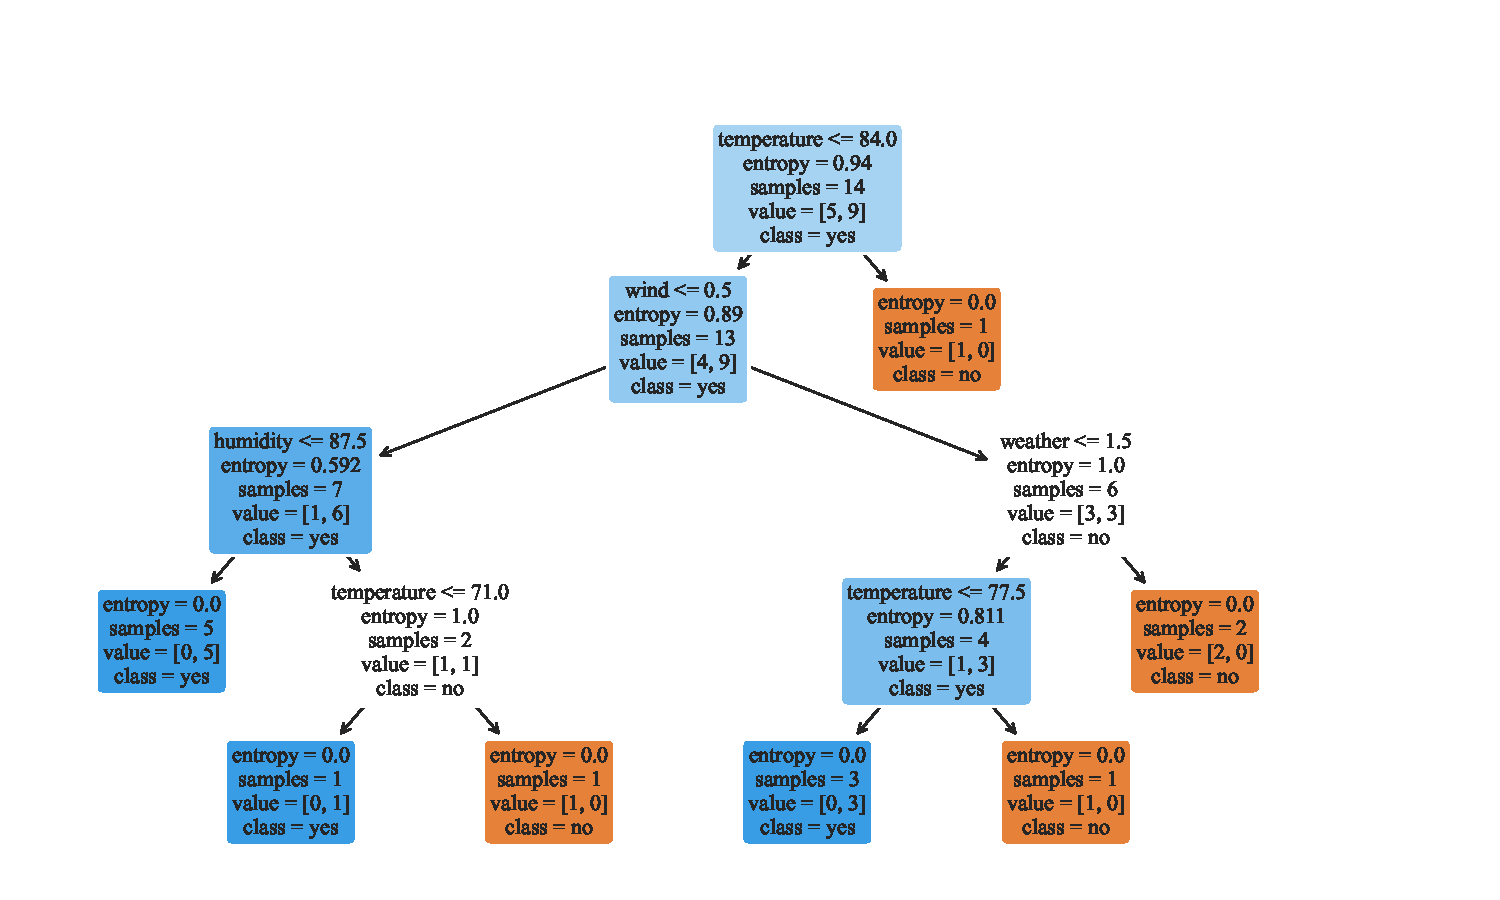
\includegraphics[width=\textwidth]{tree_result.pdf}
    \caption{决策树划分结果} \label{fig:tree_result}
\end{figure}

\includepdfset{pagecommand={\thispagestyle{fancy}}} 
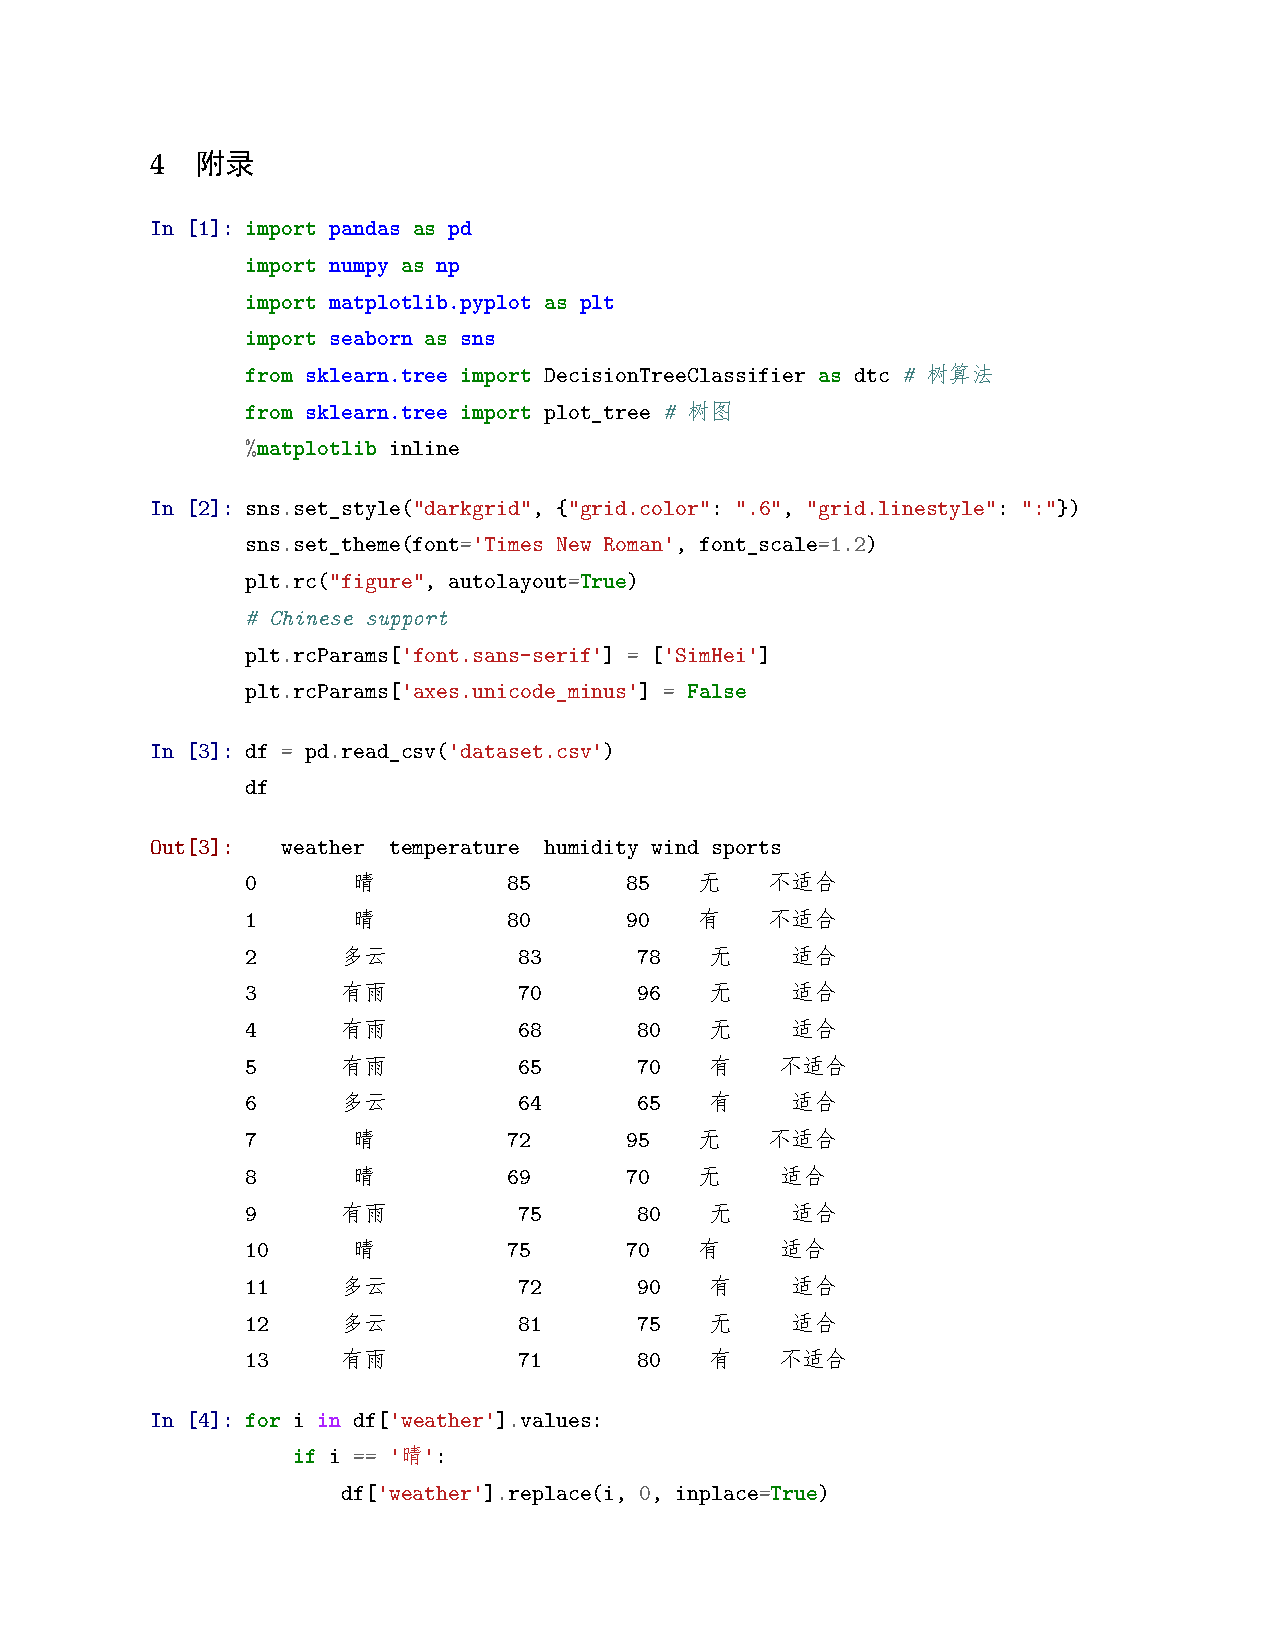
\includepdf[addtotoc={1,section,1,附录,appendix}, pages={1-3}]{DecisionTree.pdf}

% % 参考文献,此处以 MLA 引用格式为例

% \begin{thebibliography}{9}
%     \bibitem{1} Clemente, Filipe Manuel, et al. "General network analysis of national soccer teams in FIFA World Cup 2014." \emph{International Journal of Performance Analysis in Sport} 15.1 (2015): 80-96.
%     \bibitem{3} Dijkstra, Edsger Wybe. "A Note on Two Problems in Connexion With Graphs." \emph{Numerische Mathematik} 1(1959):269-271.
%     \bibitem{4} Ahnert, Sebastian E., et al. "Ensemble approach to the analysis of weighted networks.." \emph{Physical Review E} 76.1 (2007).
%     \bibitem{5} Wong, J. A. Hartiganm. A. . "Algorithm AS 136: A K-Means Clustering Algorithm." \emph{Journal of the Royal Statistical Society. Series C (Applied Statistics)} 28.1(1979):100-108.
%     \bibitem{6} Buldu, J. M., et al. "Defining a historic football team: Using Network Science to analyze Guardiola’s F.C. Barcelona." \emph{Scientific Reports} 9.1 (2019): 1-14.
%     \bibitem{7} \emph{Balotelli sends Italy past Germany}. (2012). Retrieved December 10, 2014, from\url{https://www.uefa.com/uefaeuro/season=2012/matches/round=15174/match=2003379/index.html}
%     \bibitem{8} Sigari, Mohamad Hoseyn, et al. "Counterattack detection in broadcast soccer videos using camera motion estimation." \emph{international symposium on artificial intelligence} (2015): 101-106.
%     \bibitem{9} Abdelmahmoud Hassan Elsheikh. \emph{Effect of Leadership Intensity on Integrating Some Formal and Informal Organizational Efforts for Community Development in Khartoum Province}. 2016.
% \end{thebibliography}


% \includepdf[pages={1,2}]{Memo.pdf} 
% 可以直接导入pdf页面
% \newpage
% \begin{appendices}  % 附录环境
% \section{附录}
% \end{appendices}

\end{document}  % 结束